\documentclass{beamer}

\mode<presentation> {
	\usetheme{Darmstadt}
	\usecolortheme{rose}
	\usefonttheme{professionalfonts}
	\usefonttheme[onlymath]{serif}
}

\usepackage{ulem}
\usepackage{graphicx}
\usepackage{booktabs}
\usepackage[UTF8,noindent]{ctexcap}
\usepackage[bookmarks=true]{hyperref}
\usepackage{amsmath, amssymb}
\usepackage{mathtools}
\usepackage{array}
\usepackage{listings}
\usepackage{xcolor}

\setlength{\parskip}{0.6em}

\lstset{
	basicstyle=\ttfamily\scriptsize,
	breaklines=true,
	breakatwhitespace=false,
	columns=fullflexible,
	keepspaces=true,
	showstringspaces=false,
	tabsize=2
}

\title[浅谈 PageRank 算法]{浅谈 PageRank 算法} 

\author % Your name
{
	\small
	{
		唐怡 \and
		姚鑫婷 \and
		李知夏
	}
}

\institute[] % 您的机构将出现在每张幻灯片的底部，可能是节省空间的简写
{
	湖南大学 \space 计算机学院 \\ % 你所在的机构
	\medskip
}
\date{\today} % 日期，可以更改为自定义日期

\begin{document}

\begin{frame}
	\titlepage
\end{frame}

\section{1. 算法过程}

\begin{frame}
	\frametitle{1.1 图上随机游走}
	PageRank 将网页之间的引用关系视为一个有向图，这是一个在图上跑的算法。
\end{frame}

\begin{frame}
	\frametitle{1.1 图上随机游走}
\begin{columns}[T]
	\begin{column}{0.48\textwidth}
		\begin{center}
			% 左侧图片可能原始尺寸较大：用高度上限 + keepaspectratio 避免撑爆整页
			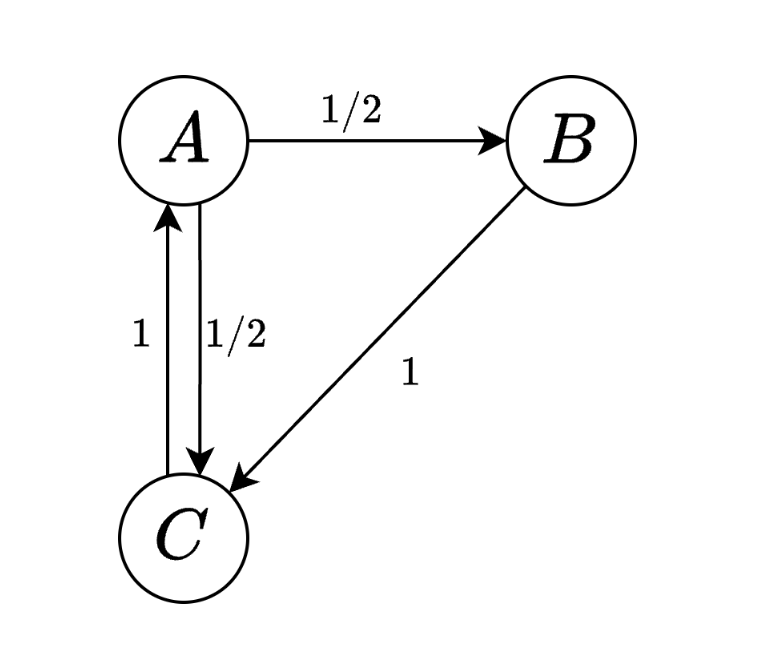
\includegraphics[width=\linewidth,height=0.55\textheight,keepaspectratio]{images/random-walk.png}
		\end{center}
	\end{column}
	\begin{column}{0.52\textwidth}
		\raggedright
		PageRank 认为浏览者是在网页上进行随机游走的，对应到有向图上，就是在有向图上随机游走。
		
		\pause
		
		由于是随机游走，所以从一个节点出发，到达相邻节点的概率是相同的。
	\end{column}
\end{columns}
\end{frame}

\begin{frame}
	\frametitle{1.1 图上随机游走}
	记 \(p_{i,j}\) 为第 \(i\) 轮后，位于节点 \(j\) 的概率。

	初始时，位于每个节点的概率相同，即 \(p_{0,i} = \frac{1}{n}\)。

	\pause

	从第 \(i\) 轮到第 \(i+1\) 轮，有状态转移：
	\[
	p_{i+1, v} = \sum_u p_{i, u} \cdot T_{u,v}
	\]
\end{frame}

\begin{frame}
	\frametitle{1.1 图上随机游走}
	该过程可以用矩阵表示。比如上图的例子，转为矩阵表示：
	\[
	\mathbf{G} = \begin{bmatrix}
		0 & 1 & 1 \\
		0 & 0 & 1 \\
		1 & 0 & 0
	\end{bmatrix}
	\]
	\pause
	按行归一化，则得到从一个点出去到别的点的概率：
	\[
	\mathbf{T} = \begin{bmatrix}
		0 & \frac{1}{2} & \frac{1}{2} \\
		0 & 0 & 1 \\
		1 & 0 & 0
	\end{bmatrix}
	\]
\end{frame}

\begin{frame}
	\frametitle{1.1 图上随机游走}
	初始时我们有行向量，表示位于各个节点的概率：
	\[
	\mathbf{V} = \begin{bmatrix}
		\frac{1}{3} & \frac{1}{3} & \frac{1}{3}
	\end{bmatrix}
	\]
	\pause
	行向量乘以矩阵会得到一个新的行向量。矩阵乘法的过程和上述状态转移含义相同：
	\[
	\mathbf{V}\mathbf{T}=
	\begin{bmatrix}
		\frac{1}{3} & \frac{1}{3} & \frac{1}{3}
	\end{bmatrix}
	\begin{bmatrix}
		0 & \frac{1}{2} & \frac{1}{2} \\
		0 & 0 & 1 \\
		1 & 0 & 0
	\end{bmatrix}
	= 
	\begin{bmatrix}
		\frac{1}{3} & \frac{1}{6} & \frac{1}{2}
	\end{bmatrix}
	=\mathbf{V}'
	\]
\end{frame}

\begin{frame}
	\frametitle{1.1 图上随机游走}
	于是，我们不断地右乘矩阵 \(\mathbf{T}\)，即可得到一直随机游走后，到达每个节点的概率。
	
	\pause
	
	我们将每个节点的概率从大到小排，就相当于完成了对节点的排名。
\end{frame}

\begin{frame}
	\frametitle{1.2 等级泄露}
	等级泄露指的是，如果有节点出度为 \(0\)，则意味着概率会不断地累积到这个节点。那么随着这个随机游走的过程不断进行下去，这个节点会不断地”吸干“别的节点的权重。
	
	\pause
	
	我们将出度为 \(0\) 的节点称为 \(\text{dangling node}\)，其组成集合为 \(\text{danglingNodes}\)。
	
	\pause
	
	走不出去的概率：
	\[
	leakRank = \sum_{i\in \text{danglingNodes}}{\mathbf{V}_i}
	\]
\end{frame}

\begin{frame}
	\frametitle{1.2 等级泄露}
	PageRank 算法考虑，如果一个人浏览到一个没有另外跳转链接的页面，那么这个人下一步可能会随机跳转到所有的界面上。
	
	\pause

	我们这种随机跳转时，每个节点的权重组成行向量 \(\mathbf{danglingWeights}\)，那么就相当于，将 \(leakRank\) 按权重 \(\mathbf{danglingWeights}\) 重新分配。
	
	\pause

	于是原本的 PageRank 算法为：
	\[
	\mathbf{V}\mathbf{T} + leakRank \cdot \mathbf{danglingWeights} = \mathbf{V}'
	\]
\end{frame}

\begin{frame}
	\frametitle{1.3 等级沉默}
	如果一个点入度为 \(0\)，则没有节点传给他概率，那么随着随机过程的进行，这个节点的权重会归零。
	
	\pause
	
	PageRank 算法提出了一个常数因子 \(followingProb\)（又称为阻尼系数，常见取值为 \(0.85\)），表示用户有多少概率会从当前节点上继续跳转到其他节点。
	
	\pause
	
	那么 \(1 - followingProb\) 就表示用户有多少概率会跳转到一个随机的节点。
\end{frame}

\begin{frame}
	\frametitle{1.3 等级沉默}
	对于后者，随机跳转时每个节点也会有一个权重，每个节点的权重组成行向量 \(\mathbf{personalization}\)。
	
	\pause
	
	于是原本的 PageRank 算法为：
	\begin{equation*}
		\resizebox{0.95\linewidth}{!}{$
			followingProb \cdot ( \mathbf{V}\mathbf{T} + leakRank \cdot \mathbf{danglingWeights}) + (1 - followingProb) \cdot \mathbf{personalization} = \mathbf{V}'
		$}
	\end{equation*}
\end{frame}

\begin{frame}
	\frametitle{1.4 算法收敛}
	可以证明，PageRank 算法是可以收敛的。
\end{frame}

\begin{frame}
	\frametitle{1.4 算法收敛}

	\begin{equation*}
		\resizebox{0.95\linewidth}{!}{$
			followingProb \cdot ( \mathbf{V}\mathbf{T} + leakRank \cdot \mathbf{danglingWeights}) + (1 - followingProb) \cdot \mathbf{personalization} = \mathbf{V}'
		$}
	\end{equation*}

	\pause
	
	如果我们要证明上式收敛，那么只需要证明 \(\mathbf{V}\mathbf{T}\) 在这个算法过程中收敛。 
	
	\pause

	\((1 - followingProb) \cdot \mathbf{personalization}\) 是常数
	
	\pause

	对于 \(leakRank \cdot \mathbf{danglingWeights}\) 部分，我们可以不严谨地认为，假如说 \(\mathbf{V}\mathbf{T}\) 收敛了，那么 \(leakRank \cdot \mathbf{danglingWeights}\) 部分也就是常数了。 
\end{frame}

\begin{frame}
	\frametitle{1.4 算法收敛}

	\(\mathbf{V}\mathbf{T}\) 可以看成是一个马尔科夫链过程
	
	\pause
	
	\(\mathbf{V}_{\infty} = \lim_{n\to\infty}\mathbf{V}_0\mathbf{T}^n\)。\(\mathbf{V}_{0}\) 为初始时各个节点的 PageRank 值。
	
	\pause

	现在证明 \(\lim_{n\rightarrow \infty} \mathbf{T}^n\) 是收敛的。
	
\end{frame}

\begin{frame}
	\frametitle{1.4 算法收敛}
	考虑将矩阵 \(\mathbf{T}\) 做特征值分解：
	\[
	\mathbf{T}=\mathbf{X}\Lambda \mathbf{X}^{-1}
	\]

	\pause

	然后有：
	\[
	\mathbf{T}^n = \mathbf{X}\Lambda^n \mathbf{X}^{-1}
	\]

	\pause

	于是考虑 \(\Lambda^n\) 的收敛性。\(\Lambda\) 是对角矩阵。主对角线上的元素是由 \(\mathbf{T}\) 的特征值组成的。
	
	\pause

	事实上，\(\mathbf{T}\) 的特征值 \(\lambda_i\) 必然满足 \(|\lambda_i|\le 1\)，于是 \(\Lambda^n\) 是收敛的。
\end{frame}

\begin{frame}
	\frametitle{1.4 算法收敛}
	下面证明 \(\mathbf{T}\) 的特征值 \(\lambda_i\) 必然满足 \(|\lambda_i|\le 1\)：
	
	\pause

	我们称 \(\mathbf{T}\) 为马尔可夫矩阵，当且仅当它每一行的元素之和为 \(1\)
	
	\pause

	\begin{itemize}
		\item 我们这里是右乘马尔可夫矩阵，所以要求每一行之和为 \(1\) \pause
		\item 矩阵中每一项都是概率，\(0\le \mathbf{T}_{ij} \le 1\) \pause
		\item 简单起见，这里不考虑 dangling nodes。
	\end{itemize}

	\pause

	易知：两个马尔可夫矩阵相乘，结果也是马尔可夫矩阵。
\end{frame}

\begin{frame}
	\frametitle{1.4 算法收敛}
	令 \(\mathbf{T}\) 中绝对值最大的特征值为 \(\lambda_1\)，其对应的特征向量为 \(\mathbf{x}\)，根据特征值定义，有：
	\[
	\mathbf{T}\mathbf{x} = \lambda_1\mathbf{x}
	\]

	\pause

	于是有：
	\begin{align*}
	\mathbf{T}^n\mathbf{x}
	&= \mathbf{T}^{n-1}\cdot \mathbf{T} \cdot \mathbf{x} \\
	&= \mathbf{T}^{n-1}\cdot \lambda_1 \mathbf{x} \\
	&= \lambda_1 \mathbf{T}^{n-1}\cdot  \mathbf{x} \\
	&\cdots \\
	&=\lambda_1^n\mathbf{x}
	\end{align*}
\end{frame}

\begin{frame}
	\frametitle{1.4 算法收敛}
	假如说 \(|\lambda_1|>1\)，那么 \(\lim_{n\rightarrow \infty}\lambda_1^n\mathbf{x} = \infty\)。

	\pause
	
	而 \(\mathbf{T}^n\) 的每个元素都是位于 0 和 1 之间的，所以显然趋近不了无穷，因此假设不成立。

	\pause

	所以 \(\mathbf{T}\) 的特征值 \(\lambda_i\) 必然满足 \(|\lambda_i|\le 1\)。
\end{frame}

\begin{frame}
	\frametitle{1.4 算法收敛}
	如何判定收敛？

	\pause
	
	Talk is cheap, show me your code.
\end{frame}

\begin{frame}
	\frametitle{1.5 时间复杂度}
	令矩阵运算的时间复杂度为 \(M\)，迭代次数为 \(d\)，那么时间复杂度就为 \(dM\)。 \pause

	\(M\)？视代码实现而定。 \pause

	\(d\)？

	\pause

	\begin{itemize}
		\item 有人说是 \(\log\) 级别的（通过实验得出的结果）。 \pause
		\item 我们在实际中发现，迭代次数是比较小的，一般来说可能个位数的迭代次数就差不多了。 \pause
		\item 我们随后又发现，迭代次数和 \(followingProb\) 有关，\(followingProb\) 比较大的话，迭代次数也会变得比较多。
	\end{itemize}
\end{frame}

\section{2. 代码实现}

\begin{frame}
	\frametitle{2. 代码实现}
	GitHub：https://github.com/caiwen666/hnu-algo
\end{frame}

\begin{frame}
	\frametitle{2.1 朴素实现}
	我们使用 Rust。考虑到矩阵乘法的实现并不是该算法的重点，我们直接使用 Rust 的 ndarray crate 进行矩阵运算： \pause

	不过建图时有一个细节需要注意，如果 \(u\) 向 \(v\) 有重边，那么 \(\mathbf{G}_{u,v}\) 还是为 \(1\)。
\end{frame}

\begin{frame}[fragile]
	\frametitle{2.1 朴素实现}
\begin{lstlisting}
pub fn rank(&self, following_prob: f64, tolerance: f64) -> Vec<(T, f64)> {
	...
    // 初始化 PageRank
    let mut last = Array2::<f64>::from_elem((1, self.capacity), 1.0 / self.capacity as f64);
    let personalization = last.clone();
    let dangling_weights = personalization.clone();
    // 不断迭代直到达到收敛条件
    loop {
        let t = last.select(Axis(1), dangling_nodes_index.as_slice());
        let leak_rank = t.sum();
        let current = following_prob
            * (last.dot(&transition_matrix) + leak_rank * &dangling_weights)
            + (1.0 - following_prob) * &personalization;
        // CALLBACK: 收敛判定
        if (&last - &current).abs().sum() < self.capacity as f64 * tolerance {
            break;
        }
        last = current;
    }
	...
}
\end{lstlisting}
\end{frame}

\begin{frame}
	\frametitle{2.1 朴素实现}
	我们在三体人物关系的图上跑了一下 PageRank 算法。 \pause

	数据来源：https://textdata.cn/blog/2022-11-29-santi-relationship-visualization-with-pyecharts/ \pause

	测试代码在 \texttt{/tests/pagerank.rs} 中。
\end{frame}

\begin{frame}[fragile]
	\frametitle{2.1 朴素实现}
\begin{lstlisting}
[("罗辑", 0.06317139467552539), ("叶文洁", 0.06088064117254309), ("程心", 0.05211684856535334), ("汪淼", 0.04618440510334715), (" 云天明", 0.0407062044364546), ("智子", 0.035534663924738), ("章北海", 0.024534285949243787),
...
\end{lstlisting}
	\pause

	从直觉上来看是没问题的，众所周知罗辑是三体中的核心人物... 
	
\end{frame}

\begin{frame}[fragile]
	\frametitle{2.1 朴素实现}

	不过我们还有另一个思考：如果我们直接把图上节点按度数（原图是无向图）从大到小排序，貌似也能得到一个差不多的：

	\pause

\begin{lstlisting}
[('叶文洁', 34), ('罗辑', 34), ('程心', 28), ('汪淼', 26), ('云天明', 22), ('智子', 20), ('史强', 12), ('章北海', 12),
...
\end{lstlisting}

	\pause

	在这个数据集上，PageRank 的效果看起来并没有很显著。 
	
	\pause

	直观地理解，PageRank 通常用来缓解这种情况：如果一个节点被很多节点引用，但这些引用它的节点都不重要，那么即使它被引用得很多，重要性也不高。而对于三体人物，重要的人物能接触到的人自然更多，不重要的人物能接触到的人也更少。
\end{frame}

\begin{frame}
	\frametitle{2.1 朴素实现}
	我们还在一个神秘的数据集上跑了一下 PageRank：

	\pause

	数据来源：https://snap.stanford.edu/data/web-Google.html

	\pause

	网站上说这是 Google 搜索引擎爬取到的真实的网站引用关系的数据，但他把网站链接映射成编号了，趣味性有点低...
\end{frame}

\begin{frame}
	\frametitle{2.1 朴素实现}
	然后不出意外 OOM 了，这个数据集有 875713 个点，我们肯定是存不下 \(875713 \times 875713\) 大小的二维数组的。
\end{frame}

\begin{frame}
	\frametitle{2.1 朴素实现}
	CALLBACK：行向量乘矩阵的时间复杂度为 \(O(n^2)\)。
\end{frame}

\begin{frame}
	\frametitle{2.2 稀疏矩阵}
	注意到，该数据集上只有 5105039 条边，远小于 \(875713 \times 875713\)，这个图很稀疏。

	\pause

	稀疏矩阵乘法的技巧详情可以参考：https://www.caiwen.work/post/mit6172-1\#1-5-sparsity

	\pause

	由于我们是行向量乘矩阵，这里我们把列压缩掉。
\end{frame}

\begin{frame}[fragile]
	\frametitle{2.2 稀疏矩阵}
\begin{lstlisting}
// algorithms/matrix.rs
pub struct CSCMatrix<T> {
    col_elements: Vec<HashMap<usize, T>>,
    row: usize,
    col: usize,
}

pub fn left_mul(&self, vector: Vec<T>) -> Vec<T> {
    if vector.len() != self.row {
        panic!("Vector length must be equal to matrix row");
    }
    let mut result = vec![T::default(); self.col];
    for (col, col_list) in self.col_elements.iter().enumerate() {
        for (row, value) in col_list.iter() {
            result[col] = result[col] + vector[*row] * *value;
        }
    }
    result
}
\end{lstlisting}
\end{frame}

\begin{frame}
	\frametitle{2.2 稀疏矩阵}
	我们只对非 \(0\) 元素进行存储并运算。非 \(0\) 元素的数量大概是边数 \(m\)，于是：
	\begin{itemize}
		\item 空间复杂度：\(O(n^2)\rightarrow O(m)\)
		\item 时间复杂度：\(O(n^2)\rightarrow O(nm)\)
	\end{itemize}
\end{frame}

\begin{frame}
	\frametitle{2.2 稀疏矩阵}

	然后再跑一下上述的 Google 的数据集，我们得到：

	\begin{tabular}{lll}
		\toprule
		节点 & PageRank 值 & 入度度数排名 \\
		\midrule
		163075 & 0.0009521123333770586 & 7 \\
		597621 & 0.0009013686628242723 & 2 \\
		537039 & 0.000895381572659312 & 1 \\
		837478 & 0.0008761661604315241 & 10+ \\
		885605 & 0.0008216087428297469 & 6 \\
		\bottomrule
	\end{tabular}

	\pause

	可以发现 PageRank 算法确实有区别于直接按度数排序的方法。
\end{frame}

\begin{frame}
	\frametitle{2.3 Something fun}
	（声明：下面的时间数据是随手测的，没有非常严格地测量。没有特殊说明的话，测试数据集均为上面 Google 的数据集）

	\pause

	我们手搓的稀疏矩阵乘法又 \texttt{Vec} 又 \texttt{HashMap}，还没上并行化，看起来速度应该是打不过经过工业级优化的 NumPy 的。
	
	\pause

	但是实际测试下：
	\begin{itemize}
		\item Rust 手搓：1.0029702s
		\item NetworkX（基于 scipy 和 numpy）：6.83s
	\end{itemize}

\end{frame}

\begin{frame}[fragile]
	\frametitle{2.3 Something fun}
	理论上 NumPy 是基于 C/C++ 的，不应该打不过 Rust。我们猜想，可能即使矩阵乘法那一块加速了，但是 Python 本身还是比较拉跨。
	
	\pause
	
	比如 NetworkX 实现的 PageRank 算法在最后进行了一个数据转换：

\begin{lstlisting}
return dict(zip(nodelist, map(float, x)))
\end{lstlisting}

	\pause

	这个过程大概有 0.25s 的开销。

\end{frame}

\begin{frame}
	\frametitle{2.3 Something fun}
	同时我们在分析性能差距的时候偶然发现 NetworkX 有两处向量元素求和用的是 Python 自带的 \texttt{sum()}，而不是 NumPy 的 \texttt{sum()}。
	
	\pause
	
	后者理论上应该会存在优化。
\end{frame}

\begin{frame}[fragile]
	\frametitle{2.3 Something fun}
\begin{lstlisting}
start = time.perf_counter()
sum1 = np.sum(x[is_dangling])
sum_time1 = time.perf_counter() - start
start = time.perf_counter()
sum2 = sum(x[is_dangling])
sum_time2 = time.perf_counter() - start
start = time.perf_counter()
sum3 = sum(x[is_dangling])
sum_time3 = time.perf_counter() - start
start = time.perf_counter()
sum4 = np.sum(x[is_dangling])
sum_time4 = time.perf_counter() - start
print(f"Sum Time: {sum_time1:.10f} seconds, {sum_time2:.10f} seconds, {sum_time3:.10f} seconds, {sum_time4:.10f} seconds")
\end{lstlisting}
\end{frame}

\begin{frame}[fragile]
	\frametitle{2.3 Something fun}
\begin{lstlisting}
Sum Time: 0.0007621000 seconds, 0.0040127000 seconds, 0.0037306000 seconds, 0.0005124000 seconds
Sum Time: 0.0008018000 seconds, 0.0041156000 seconds, 0.0040253000 seconds, 0.0007563000 seconds
\end{lstlisting}

	\pause

	测试结果表明使用 NumPy 的 \texttt{sum()} 大概会有 3 到 4 倍的提升。
\end{frame}

\begin{frame}
	\frametitle{2.3 Something fun}
	因此我们顺手贡献了一下代码（现已合并到主分支）：
	\begin{center}
		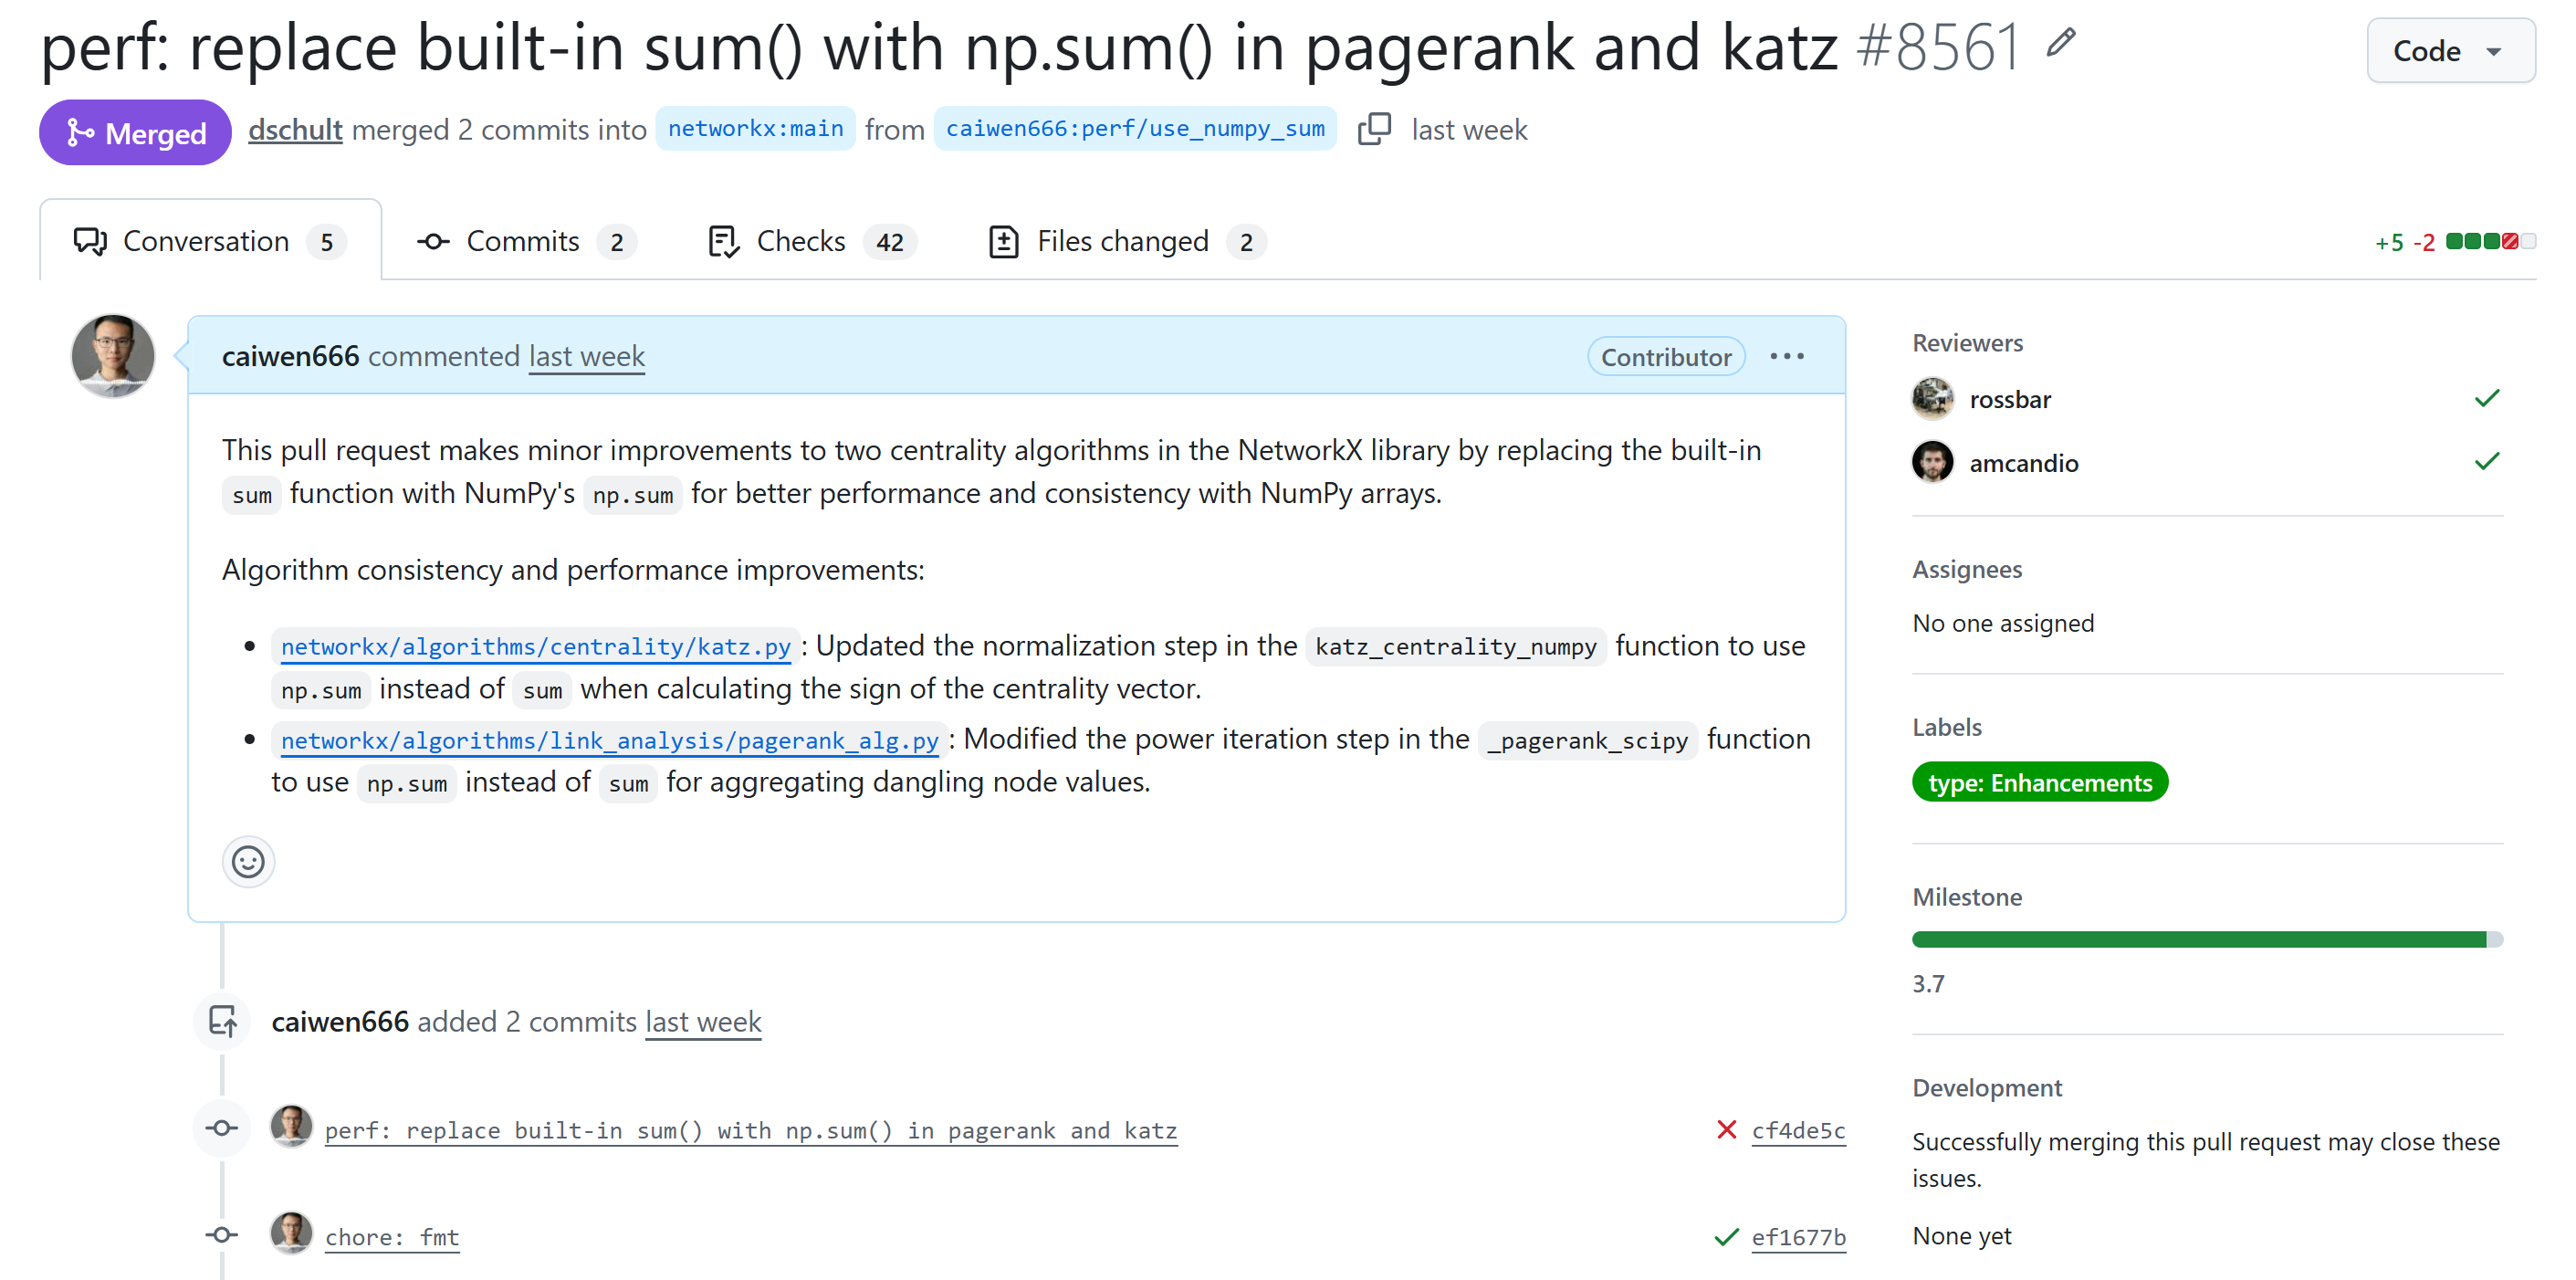
\includegraphics[width=0.92\linewidth]{images/networkx-pr.png}
	\end{center}
\end{frame}

\begin{frame}
	\frametitle{2.3 Something fun}
	我们在腾讯云计算型 C4 实例上进行了非常粗糙的性能测试。

	\pause

	方法和对比结果在 https://github.com/networkx/networkx/pull/8561

	\pause
	
	在 https://snap.stanford.edu/data/ego-Twitter.html 的数据集上，通过设置 \texttt{alpha=0.99}，即上文的 \(followingProb\)，\texttt{tol=1e-12}，即上文的 \(tolerance\)，人为地把迭代次数拉高到了 1135。
	
	\pause

	获得了大概 10\% 的性能提升。
\end{frame}

\section{3. 应用}

\begin{frame}
	\frametitle{3. 应用}
	PageRank 本质上还是图上权重的传播。通过将要分析的东西构造成图，以及设置 \(\mathbf{V}_0\)、\(\mathbf{danglingWeights}\)、\(\mathbf{personalization}\) 等参数，可以发挥出不同的作用。
\end{frame}

\begin{frame}
	\frametitle{3.1 TrustRank}
	TrustRank 用于检测垃圾网站。

	\pause

	TrustRank 基于这样一个观察：权威的网站一般不会指向垃圾网站。所以 TrustRank 算法先挑选一些完全可以信任的网站，将这些网站的 TrustRank 的值设为最高，其他网站的 TrustRank 通过这些网站的 TrustRank 值传播得到。

\end{frame}

\begin{frame}
	\frametitle{3.1 TrustRank}
	设选择了 \(n\) 个完全信任的网站，那么：
	\[
	\mathbf{V}_0(i) = \mathbf{personalization}(i) =
	\begin{cases}
		\frac{1}{n} &,\text{i 为完全信任的网站} \\
		0 &,\text{otherwise}
	\end{cases}
	\]
\end{frame}

\begin{frame}
	\frametitle{3.1 TrustRank}
	Anti-TrustRank：反过来做，标记垃圾网站，然后从垃圾网站逆向传播权重。
\end{frame}

\begin{frame}[fragile]
	\frametitle{3.2 TextRank}
	TextRank 算法用于给文本内的词计算排名，可以统计文本的关键字，生成摘要。

	\pause

	首先先把文本进行分词，比如：

	\pause

\begin{lstlisting}
党中央决定，在全党开展树立和践行正确政绩观学习教育，这是今年党的建设的重要任务
\end{lstlisting}

	\pause

\begin{lstlisting}
['党中央', '决定', '，', '在', '全党', '开展', '树立', '和', '践行', '正确', '政绩观', '学习', '教育', '，', '这是', '今年', '党的建设', '的', '重要', '任务']
\end{lstlisting}
\end{frame}

\begin{frame}[fragile]
	\frametitle{3.2 TextRank}
	分词会分出来一些标点符号和无关紧要的词（比如“的”、“和”这种）。我们的实现是直接把长度为 1 的词全部过滤掉：

	\pause

\begin{lstlisting}
['党中央', '决定', '全党', '开展', '树立', '践行', '正确', '政绩观', '学习', '教育', '这是', '今年', '党的建设', '重要', '任务']
\end{lstlisting}
\end{frame}

\begin{frame}[fragile]
	\frametitle{3.2 TextRank}
	算法有一个参数 \(windowSize\)。我们在分词出来的序列上从左到右用大小为 \(windowSize\) 的窗口扫描，然后把窗口内的词两两建立无向边。
	
	\pause

	比如 \(windowSize = 2\) 时，会建立如下的边：

\begin{lstlisting}
党中央 <-> 决定
决定 <-> 全党
全党 <-> 开展
...
\end{lstlisting}

	\pause

	然后就可以得到一张图，对这个图跑 PageRank 就得到了 TextRank。
\end{frame}

\begin{frame}
	\frametitle{3.2 TextRank}
	我们测试了一下效果，在 http://dangjian.people.com.cn/n1/2026/0225/c117092-40669694.html 这篇文章上做 \(windowSize = 3\) 的 TextRank，得到结果：

	\pause

	\begin{tabular}{lll}
		\toprule
		词 & TextRank & 词频排名(词频) \\
		\midrule
		教育 & 0.01689736222299958 & 2(14) \\
		学习 & 0.015962592072431534 & 2(14) \\
		坚持 & 0.01435974021719568 & 7(8) \\
		人民 & 0.013646755229879898 & 7(8) \\
		政绩观 & 0.013452460045266328 & 1(15) \\
		\bottomrule
	\end{tabular}
\end{frame}

\begin{frame}
	\frametitle{3.2 TextRank}
	然后又在某个小作文上面跑了一遍 \(windowSize = 3\) 的 TextRank
	\begin{center}
		
\includegraphics[width=0.92\linewidth]{images/textrank-demo.png}
	\end{center}
\end{frame}

\begin{frame}
	\frametitle{3.2 TextRank}
	得到结果：

	\begin{tabular}{lll}
		\toprule
		词 & TextRank & 词频排名(词频) \\
		\midrule
		我们 & 0.024564948289610245 & 1(44) \\
		没有 & 0.008737309221451349 & 4(14) \\
		放假 & 0.007786354788189854 & 2(15) \\
		什么 & 0.0072075023195175515 & 2(15) \\
		\bottomrule
	\end{tabular}
\end{frame}

\begin{frame}
	\frametitle{3.2 TextRank}
	TextRank 还可以通过搞什么余弦相似度来把句子之间建图，生成文章摘要。不过我们不太感兴趣了。现在我们随便调用一下大模型就能得到更优的结果。
	
	\pause

	比如上面的关键字丢给大模型：

	\begin{center}
		
\includegraphics[width=0.92\linewidth]{images/llm-keywords.png}
	\end{center}
\end{frame}

\begin{frame}
	\frametitle{3.2 TextRank}
	TextRank 的代码实现在代码仓库的 \texttt{src/bin/text\_rank.rs} 里，感兴趣的可以玩玩。
\end{frame}

\section{END}

\begin{frame}
	\Huge{\centerline{THANK YOU!}}
\end{frame}

\end{document}

